\section{Red or Blue?}

Boolean satisfiability (SAT)  is, as far as  Computer Scientists know, a  hard problem. We
will define precisely what we mean by `hard', later on in the course. This problem is defined
as follows:
\begin{center}
	\fbox{
		\begin{minipage}{6in}
			The input  is a  collection of  $m$ \emph{clauses} over  $n$ boolean  variables $X_1$,
			$X_2$, \ldots $X_n$.  Each clause is a  disjunction of some of the  variables or their
			complements.\vskip8pt

			The problem consists in answering the question ``Is there a way to assign truth values
			to each variable that makes \textbf{every} clause of the instance \textsc{True}?'' (For short this is called a {\em valid truth assignment}.)
		\end{minipage}}
\end{center}
For instance, here is an instance of SAT made of 4 clauses over 3 variables:
\begin{displaymath}
	\begin{array}{rrl}
		\hbox to 20pt{\hfil} & 1. & X_1 \lor \overline{X}_3                     \\
		                     & 2. & \overline{X}_1 \lor \overline{X}_2 \lor X_3 \\
		                     & 3. & \overline{X}_2 \lor \overline{X}_3          \\
		                     & 4. & X_3                                         \\
	\end{array}
\end{displaymath}
Equivalently, you could think of this instance as the single boolean expression
\begin{displaymath}
	\begin{array}{rl}
		\hbox to 20pt{\hfil} & (X_1 \lor \overline{X}_3) \land {}                     \\
		                     & (\overline{X}_1 \lor \overline{X}_2 \lor X_3) \land {} \\
		                     & (\overline{X}_2 \lor \overline{X}_3) \land {}          \\
		                     & X_3                                                    \\
	\end{array}
\end{displaymath}

There are  many other problems  whose level  of difficulty is  similar to that  of Boolean
Satisfiability, and this problem has attracted a  lot of research. So while the problem is
difficult to solve  in general, a number of  tools to solve instances of  the problem have
been                       developed                        (see                       the
\href{https://en.wikipedia.org/wiki/Boolean_satisfiability_problem}  {Wikipedia page}  for
details and  links). We can take  advantage of these  tools to solve other  problems using
\emph{reductions}.

In this question, we will  look at the problem of determining whether or  not a graph is a
\emph {split graph}. A graph $G = (V, E)$ is a \emph {split graph} if we can partition its
vertex set $V$ into two subsets $V_1$, $V_2$ such that $V = V_1 \cup V_2$, $V_1 \cap V_2 =
	\emptyset$, every  two vertices of  $V_1$ are  connected by an  edge ($\forall v  \in V_1,
	\forall w \in  V_1, \{ v, w \}  \in E$) and no  two vertices of $V_2$ are  connected by an
edge ($\forall  v \in V_2, \forall  w \in V_2,  \{ v, w  \} \notin E$). For  instance, the
following graph  is a split graph,  where the vertices of  $V_1$ are colored Red,  and the
vertices of $V_2$ are colored Blue.

\begin{center}
	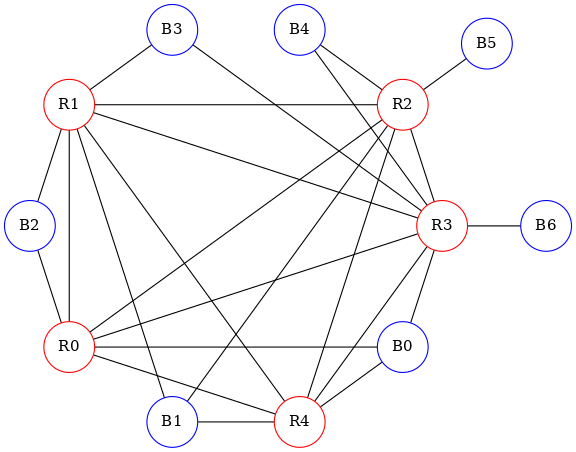
\includegraphics[width=3.8in]{split-graph.png}
\end{center}

\begin{questions}
	\question[4] Show how  to reduce an arbitrary  instance of the split  graph recognition problem
	into  an instance  of  \emph {Boolean  Satisfiability}  (SAT). (Remember that, per the problem specifications, your clauses must be in \href{https://en.wikipedia.org/wiki/Conjunctive_normal_form}{conjunctive normal form}.) Hint:  you  will want  to
	introduce a single variable for each vertex of the graph.

	\begin{soln}
		We have for any \(v_i \in V\) that either \(v_i \in V_1\) or \(v_i \in V_2\) but not both since they form a partition over \(V\).

		Then denote the boolean variable \(X_i\) so that

		\[
			X_i =
			\begin{cases}
				T, & \text{if } v_i \in V_1 \\
				F, & \text{if } v_i \in V_2
			\end{cases}
		\]

		Observe for two any vertices \(\{v_i, v_j\}\) they form an edge or do not.

		We see if \(v_i, v_j \in V_1\) then they share an edge, similarly, if \(v_i, v_j \in V_2\) then they do not share an edge.

		If two vertices share an edge, we cannot tell if both are in \(V_1\) but we know at least one is.

		Hence, for for ever edge pair, \(\{v_i, v_j\}\) the disjunction is true, \((X_i \lor X_j)\).

		Now consider pairs \(\{v_i, v_j\} \notin E\), observe if pairs do not share an edge, then both are not in \(V_1\).

		In particular, the statement \(\lnot (X_i \land X_j )\) is true for every non-edge pair, equivalently, \((\lnot X_i \lor \lnot X_j)\) holds.

		Then we construct the SAT instance,

		\[
			\left(\bigwedge_{\{v_i, v_j\} \notin E}  (\lnot X_i \lor \lnot X_j)\right) \land \left(\bigwedge_{\{v_i, v_j\} \in E}(X_i \lor X_j)\right).
		\]

		If such a solution to this SAT instance exists, then \(G\) is a split graph.
	\end{soln}

	\ifsolutions\begin{soln}
	Let \(V\) be a vertex set. Add \(v \in V\). Then also add \(v_1, v_2, \dots, v_n\) to \(V\).

	Then for \(v_1, v_2, \dots, v_d\) add \((v, v_i) \in E\) for \(i = 1, 2, \dots, d\).

	Then colour the node \(v\) blue, and colour all other nodes in \(V\) red.

	By construction, the degree of all other nodes that are not \(v\) is \(1\) since it's only connected to \(v\).

	Thus, the degree of \(v\) is the maxmimum degree of the graph, which is \(d\).

	Since no nodes are adjacent except for ones to \(v\). Then the colour red is never shared by adjacent vertices.

	Thus, this graph with maximum degree \(d\) can be coloured with two colours.

\end{soln}
\fi

	\question[1] Write the collection of clauses you would get for the following graph:

	\begin{soln}
		\[
			(\lnot X_0 \lor \lnot X_1), \quad (\lnot X_1 \lor \lnot X_4), \quad
			(\lnot X_1 \lor \lnot X_2), \quad (\lnot X_2 \lor \lnot X_3),
		\]
		\[
			(X_0 \lor  X_2), \quad
			(X_0 \lor  X_3), \quad
			(X_0 \lor  X_4), \quad
			(X_1 \lor  X_3), \quad
			(X_2 \lor  X_4), \quad
			(X_3 \lor  X_4)
		\]
	\end{soln}

	\centerline{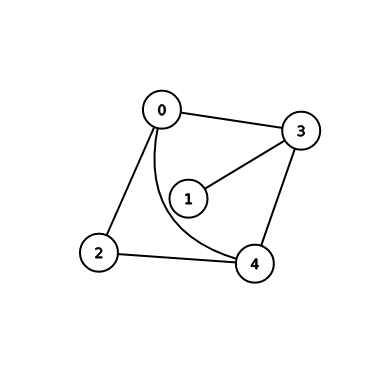
\includegraphics[width=3in]{graph1.png}}

	\ifsolutions\begin{soln}
	Proof: We provide a proof by induction on the number of nodes, \(n \in \mathbb{N}\), for graph \(G = (V, E)\).

	Base case \(|V| = 1\). The highest degree can be \(d = 0\), since the edge set would be empty.

	Thus, the algorithm uses \(1 = d + 1\) colours to colour the single node and the base case holds.

	Assume for any graph with \(n\) nodes that the algorithm will colour any ordering of nodes using at most \(d + 1\) colours.

	Consider a graph \(G = (V, E)\) with \(|V| = n + 1\) nodes with the highest degree of any node is \(d\).

	Let \(v_1, v_2, \dots, v_n, v_{n+1}\) be any ordering of the nodes. Remove \(v_{n+1}\) from this order, and the graph.

	Denote the deleted graph without \(v_{n+1}\) by \(G'\). Notice the degree of any node in \(G'\) can only decrease.

	Thus, the maximum degree of \(G'\) remains to be \(d\) with the removal of \(v_{n+1}\).

	By assumption, we can colour the ordering \(v_1, v_2, \dots, v_n\) using at most \(d+1\) colours.

	Since \(v_{n+1}\) has degree at most \(d\) then it has at most \(d\) neighbours. Then we add back \(v_{n+1}\).

	The number of colours used to colour its neigbours can be at most \(d\), if each are coloured distinctly.

	Thus, there remains at least \(1\) unique colour to colour \(v_{n+1}\) so that it is a valid colouring.

	In other words, the algorithm uses at most \(d + 1\) colours to colour the ordering \(v_1, v_2, \dots, v_{n+1}\).

	Induction makes the claim holds true for any graph with \(n\) nodes and maximum degree \(d\).


\end{soln}
\fi

	\question[3] Explain briefly why, if  an input graph is a split graph, then  there is a way to
	assign  values  to  the variables  in  the  instance  of  SAT that  makes  every  clause
	\textsc{True}.

	\begin{soln}
		If \(G = (V, E)\) is a split graph then let \(V_1, V_2\) be the respective partition as defined.

		We assign for each \(i \in V\),
		\[
			X_i =
			\begin{cases}
				T & \text{if } i \in V_1 \\
				F & \text{if } i \in V_2
			\end{cases}
		\]

		Having that \(V_1, V_2\) form a partition, this boolean variable is well defined.

		For each \(\{i, j\}\) either they form an edge or not. If they form an edge, then both cannot be in \(V_2\).

		Hence at least one is in \(V_1\), and thus, the clause \(X_i \lor X_j\) is true.

		If they are not an edge, then both are not in \(V_1\). Thus, at least one is in \(V_2\). Hence, \(\lnot X_i \lor \lnot X_j\) is true.

		Having considered every possible clause in the reduced SAT instance, we have shown this is a satisfying truth assigment, and thus the SAT is satisfiable.

	\end{soln}

	\ifsolutions\begin{soln}
	We consider the graph \(G = (V, E)\) with \(V = \{1, 2, 3, 4\}\) and \(E = \{(1, 4), (4, 3), (3, 2)\}\).

	\begin{center}
		\begin{tikzpicture}[node distance=2cm, auto]
			% Nodes
			\node[circle, draw, above  right = of 3] (1) {1};
			\node[circle, draw, right=of 1] (2) {2};
			\node[circle, draw, right=of 2] (3) {3};
			\node[circle, draw, above right=of 2] (4) {4};

			% Edges
			\draw (1) -- (4) -- (3) -- (2);
		\end{tikzpicture}
	\end{center}

	This graph can be coloured with three colours. Namely we can assign \(A = \{1, 3\}\) \(B = \{2, 4\}\).

	We see that no edges are shared between any vertices in \(A, B\) so this is a valid colouring.

	Now consider the ordering \(1, 2, 3, 4\). We first colour \(1\) blue. And then we consider \(2\).

	There is no edge between \(1, 2\) so we colour \(2\) blue and consider \(3\).

	So, its adjacent vertices have been coloured with blue, then we introduce a new colour for it red.

	Now we finally consider \(4\), its neighbours have been coloured with both red and green, so we must introduce a new colour for it purple.

	We have thus coloured this graph using three colours through the greedy algorithm when we could have used two.


\end{soln}
\fi

	\question[3] Explain briefly why,  if there is a way to assign values  to the variables in the
	instance of SAT that  makes every clause \textsc{True}, then the  graph used to generate
	the instance must be  a split graph. Show how you would determine  which vertices of $G$
	belong to which of the two subsets of $V$.

	\begin{soln}
		Suppose that we have a satisfying truth assingment to the SAT.

		Then for each assignment \(X_i\), if \(X_i\) is true, we place vertex \(i\) in \(V_1\) and if false, we place it into \(V_2\).

		We now aim to show this makes \(G\) a split graph.

		Suppose that \(i, j \in V_1\) this means that both of \(X_i, X_j\) were true.

		Hence,


	\end{soln}

	\ifsolutions\begin{soln}
\end{soln}
\fi
\end{questions}

